\documentclass{beamer}
\usetheme{Madrid}

\title{Volunteer Computing With BOINC}
\author{by Ian Palacín Aliana and Joaquim Picó Mora}
\centering
\date{November 2020}
\begin{document}
\maketitle
\begin{frame}{Content}
\begin{itemize}
\item What is Volunteer Computing? 
\item Volunteer Computing Architecture
\item What is BOINC?
\item How BOINC works?
\item Examples of Volunteer Computing
\item Minecraft@Home
\item Conclusions
\end{itemize}
\end{frame}
%
\begin{frame}{What is Volunteer Computing}
\textbf{Definition:} Is a type of distributed computing in which people donate their computers' unused resources to a research oriented project.
\begin{figure}
  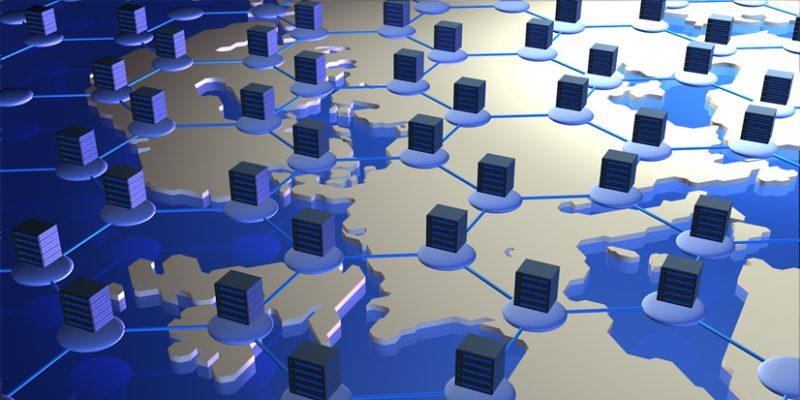
\includegraphics[width=\linewidth]{diapo1.jpg}
\end{figure}
\end{frame}

\begin{frame}{Volunteer Computing Architecture}
\begin{figure}
  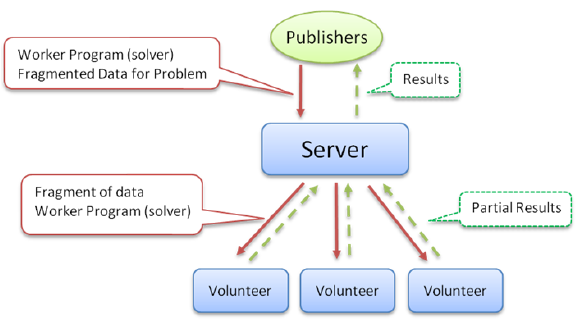
\includegraphics[width=\linewidth]{architecture.png}
\end{figure}
\end{frame}
%
\begin{frame}{What is BOINC?}
\begin{figure}
  
\includegraphics[width=\linewidth]{boinc_logo.png}
\end{figure}
\end{frame}
%
\begin{frame}{How BOINC works?}
\begin{itemize}
\item Client Workflow
\item Credit
\item How the software works
\end{itemize}
\end{frame}
%
\begin{frame}{Client Workflow}
\begin{itemize}
\item Get tasks from project \textbf{scheduling server}.
\item Download executable and input files from \textbf{data server}.
\item Run executables, producing output files.
\item Upload output files to the \textbf{data server}.
\item Report completed task to the \textbf{scheduling server}, and get new tasks.
\end{itemize}
\end{frame}
%
\begin{frame}{Credit}
\begin{figure}
  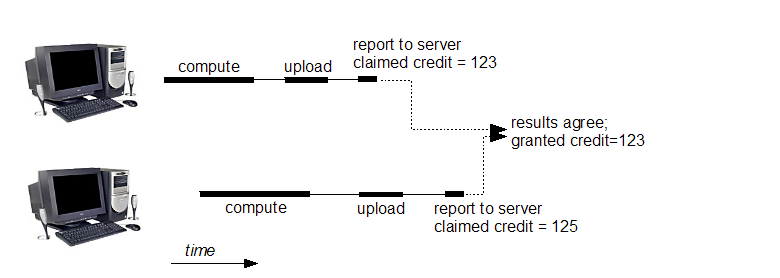
\includegraphics[width=\linewidth]{credit.png}
\end{figure}
\end{frame}
%
\begin{frame}{How the software works}
\begin{figure}
  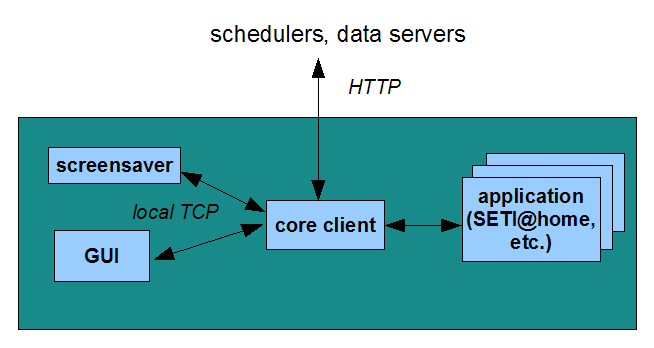
\includegraphics[width=\linewidth]{client.png}
\end{figure}
\end{frame}
\begin{frame}{Examples}
\begin{itemize}
\item \textbf{PrimeGrid:} Prime numbers
\item \textbf{Minecraft@Home:} Understanding minecraft
\item \textbf{NumberFields@Home:} Research in number Theory
\item \textbf{GPUGrid.net:} Biomedical research
\item \textbf{Einstein@Home:} Searching of weak astrophysical signals from pulsars
\item \textbf{Rosseta@Home:} Protein folding and molecular shaping
\end{itemize}
\end{frame}
%
\begin{frame}{Minecraft@Home}
\begin{itemize}
\item \textbf{Introduction}
\item The problem
\item The solution
\end{itemize}
\begin{figure}
  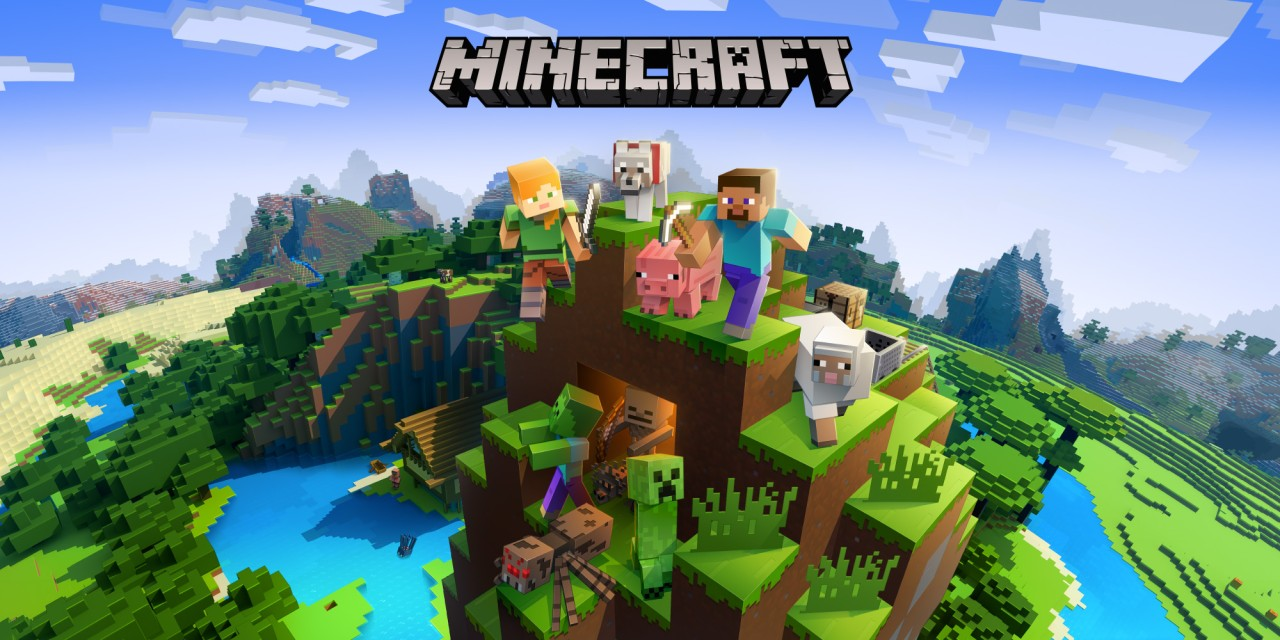
\includegraphics[scale=0.15]{minecraft.jpg}
\end{figure}
\end{frame}
\begin{frame}{Minecraft@Home}
\huge \textbf{18,446,744,073,709,551,616}
\end{frame}
%
\begin{frame}{Minecraft@Home}
\begin{itemize}
\item Introduction
\item \textbf{The problem}
\item The solution
\end{itemize}
\begin{figure}
  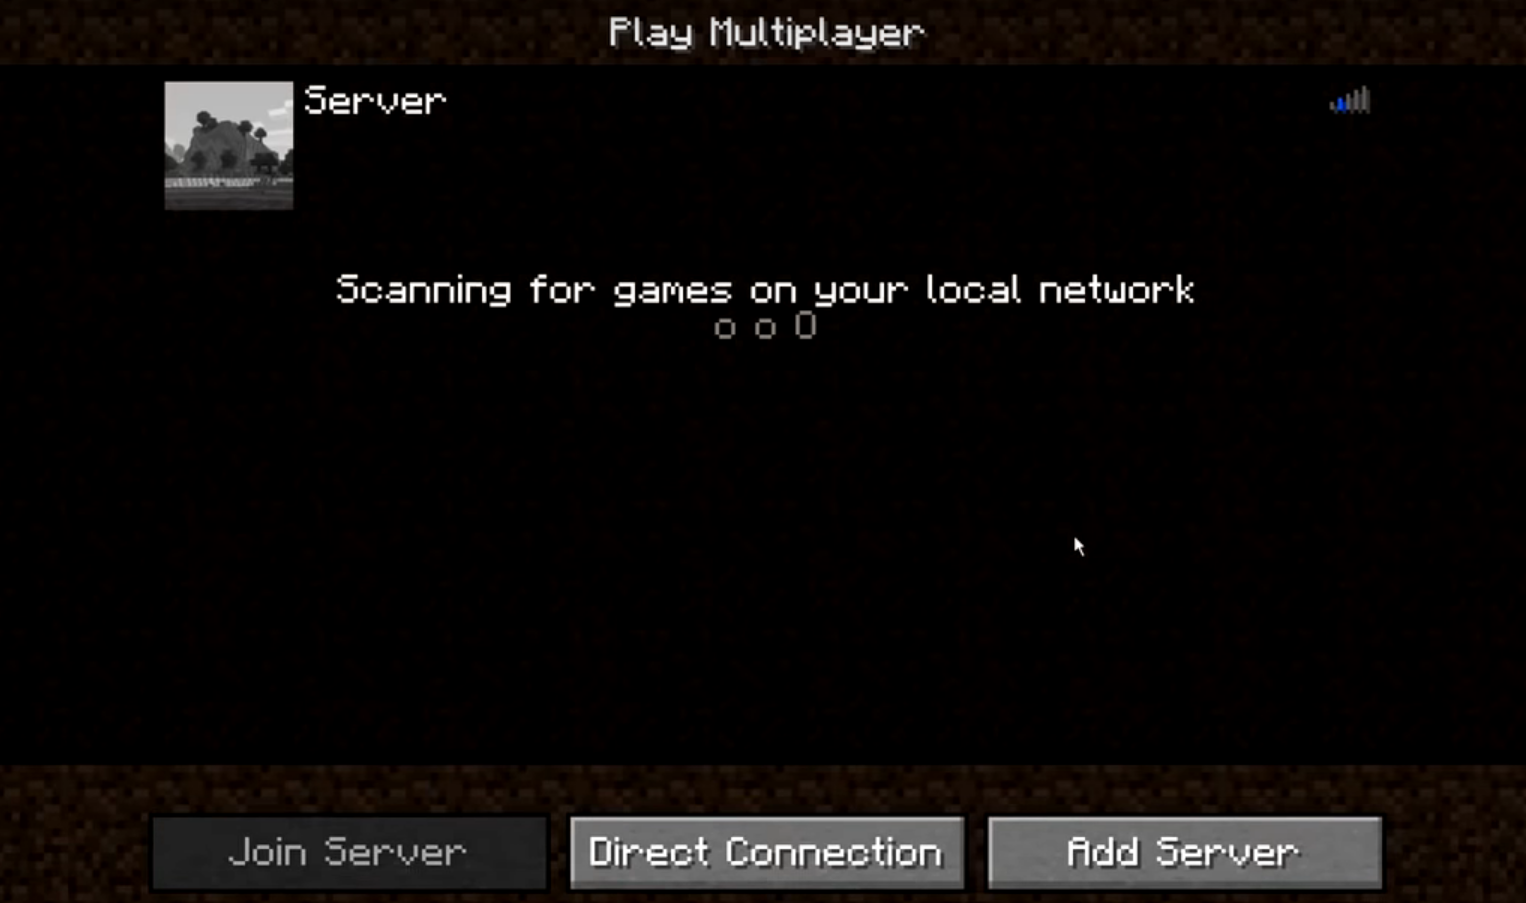
\includegraphics[scale=0.15]{pack.png}
\end{figure}
\end{frame}
%
\begin{frame}{Minecraft@Home}
\begin{figure}
  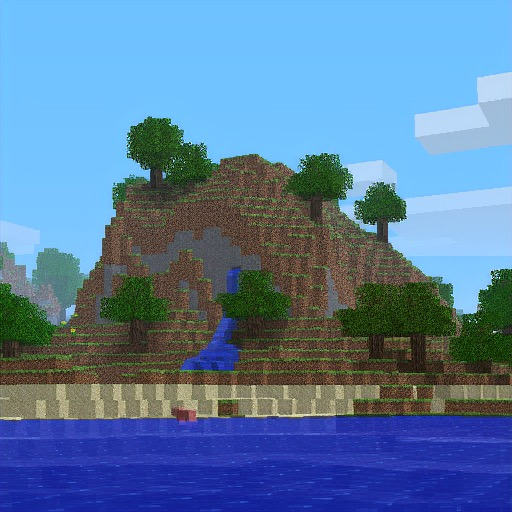
\includegraphics[scale=0.4]{pack2.jpg}
\end{figure}
\end{frame}
%
\begin{frame}{Minecraft@Home}
\begin{itemize}
\item Introduction
\item The problem
\item \textbf{The solution}
\end{itemize}
\end{frame}
%
\begin{frame}{Minecraft@Home}
\begin{figure}
  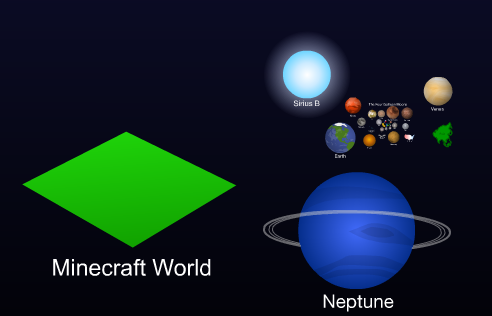
\includegraphics[width=\linewidth]{mineworld.png}
\end{figure}
\end{frame}
\begin{frame}{Advantages and Disadvantages}
\textbf{Advantages:}
\begin{itemize}
\item Can achive really big computations
\item Minimum cost 
\item The volunteers maintain their computers
\item Unlimited power
\end{itemize}
\textbf{Disadvantages:}
\begin{itemize}
\item High uncertainty
\item Low granulation
\item Unreliability, so it is needed a lot of redundancy
\item The project has to be popular
\end{itemize}
\end{frame}
\begin{frame}{Conclusions}
\huge \textbf{Final thoughts}
\end{frame}
\end{document}